\documentclass{bioinfo}
\copyrightyear{2018} \pubyear{2018}

\access{Advance Access Publication Date: Day Month Year}
\appnotes{Applications Note}

\begin{document}
\firstpage{1}

\subtitle{Subject Section}

\title[short Title]{Estimation of Structural Errors for R}
\author[Sample \textit{et~al}.]{Maik Kschischo\,$^{\text{\sfb 1,}*}$, Tobias Newmiwaka\,$^{\text{\sfb 1}}$, Benjamin Engelhardt\,$^{\text{\sfb 1}}$ and Holger Fr\"ohlich\,$^{\text{\sfb 2}}$}
\address{$^{\text{\sf 1}}$Department of Mathematics and Technology, University of Applied Sciences Koblenz RheinAhrCampus, Remagen, 53424, Germany\\
$^{\text{\sf 2}}$Algorithmic Bioinformatics, Rheinische Friedrich-Wilhelms-Universität Bonn, Bonn, 53115, Germany }

\corresp{$^\ast$To whom correspondence should be addressed.}

\history{Received on XXXXX; revised on XXXXX; accepted on XXXXX}

\editor{Associate Editor: XXXXXXX}

\abstract{
	\textbf{Motivation:} Dynamic Systems have proved to be a major tool in modelling 
	and understanding biological processes and chemical reactions. The reconstruction of 
	system states under statistical errors using e.g. Kalman Filters and Particle Filters is a 
	long discussed topic. 
	However serious issues a likely to occur as soon as the the underlying systems equations 
	contain systematic error, e.g. unknown interactions. The R package \texttt{seeds} provides 
	two algorithms that aim a numerical estimation of systematic model and simultaneously 
	estimate the system states. \\
	\textbf{Availability:} The R package \texttt{seeds} is provided via CRAN.\\
	\textbf{Contact:} \href{seeds@hs-koblenz.de}{seeds@hs-koblenz.de}
}

\maketitle

\section{Introduction}
	Cell biological interactions, chemical reactions and also mechanical systems are some 
	examples of processes that can be modelled and investigated using dynamic systems. In the 
	mathematical formulation these take the general form
	\begin{equation}
		\dot{x}(t) = f\left(x(t),u(t)\right) \label{eq:f}
	\end{equation}
	where $x(t)$ denotes the state of the system at time $t$, $u(t)$ is a known, time-
	dependent input and $f$ is a mathematical model of the system. In addition, in most 
	cases it is not possible to measure the system state $x$ directly but only 
	observables $y$ via an observation function 
	\begin{equation}
		y(t) = h\left(x(t)\right) \quad . \label{eq:h}
	\end{equation}
	It is more often the rule than the exception, that measurements $y^\text{obs}$ and 
	predictions of \eqref{eq:f} and \eqref{eq:h} do not satisfactorily coincide. If the 
	discrepancies are due to stochastic processes or measurement noise, the known methods 
	using varieties of 
	Kalman Filters and Particle Filters, to name a few, will be able to reconstruct the states 
	$x(t)$ given the data $y^\text{obs}$. As soon as the model $f$ contains systematic errors, 
	such as unknown interactions, these methods tend to fail or become very unstable. The 
	\textsc{Dynamic Elastic Net (DEN)} (\citealp{DEN}) is a dynamic optimization procedure 
	that 
	handles systematic model errors as unknown inputs to the systems equations. The methods 
	provided by \texttt{seeds} are able to optimize the unknown inputs to archive a 
	satisfactory fit to given data. Therefore these methods give a numerical estimation of 
	the model errors and at the same time estimate the true system states

\begin{methods}
\section{Methods}
	The \textsf{seeds} package provides two distinct ways to compute systematic errors. Both 
	make use of the Hamilton formalism, a convenient tool in dynamic optimization. As a setup 
	for the DEN you must provide
	\begin{enumerate}
		\item a mathematical model $f$ of the dynamic system,
		\item an observation function $h$,
		\item measured data $y^\text{obs}$. 
	\end{enumerate}
	The \texttt{greedyseeds} method is a deterministic algorithm based on a dynamic version of 
	the method of steepest descent, combined with a "greedy" selection process to archive a 
	sparse solution. In addition to the systems equations it is possible to constrain the 
	system to the solution space of algebraic equations, e.g. mass conservation. In particular 
	the case
	\begin{equation}
		\frac{\partial f_i}{\partial x_i} = 0 \quad ,
	\end{equation} 
	where the index is understood as the $i$-th component, may lead to certain numerical 
	difficulties and highly benefits of such an algebraic constraint.\\
	
	The \texttt{bayesianseeds} method is a stochastic algorithm based on bayesian 
	inference and uses LASSO regularization to generate sparsity of the solution 
	(\citealp{BDEN}). 
	In addition to a specific estimate of the unknown inputs it results in a probability 
	density in the space of unknown input functions.
\end{methods}

\section{Example}
	As an exemplary scenario we take a look at the 13-dimensional UV-B system (\citealp{UVB}) 
	and the \texttt{greedyseeds}. You can find the R notation of systems equations, 
	observation function and a data set in the package. 

	\begin{figure}[!tpb]
		\centerline{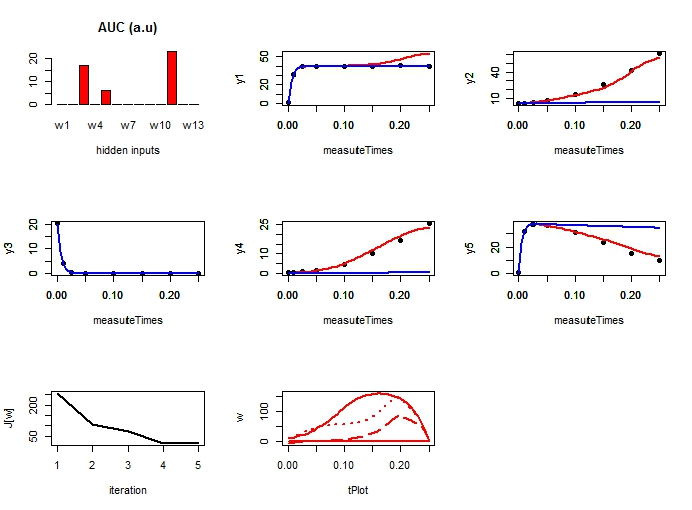
\includegraphics[width=0.5\textwidth]{Rplot.jpeg}}
		\caption{Results of the \textsf{greedyseeds} algorithm. The black markers represent 
		the data $y^\text{obs}$, the blue lines represent the erroneous model predictions and 
		the red lines show the predictions using the estimated unknown inputs $\hat{w}_i$.}
		\label{fig:example}
	\end{figure}

	Figure \ref{fig:example} shows the data and the five observables with erroneous system
	predictions as black markers and blue lines, respectively. It also shows the estimated 
	unknown inputs $\hat{w}_i$, the Area-Under-Curves and the predictions of the corrected 
	model in red. You see that the algorithm results in a sparse set of unknown inputs and how 
	the unknown inputs are able to correct the model predictions such that these fit the data.

\section{Conclusion}
	As the example shows, the R package \texttt{seeds} is able to correct systematic errors 
	in 
	dynamic model on the level of the systems equations based on optimization principles of 
	the DEN. It is able to detect the errors, and to simultaneously estimate the errors and 
	the system state. We want to point out that, depending on the properties of the system, 
	cases may occur where error are not observable. However the provided algorithms have 
	proven to yield good results in various realistic problems and may be a fruitful tool 
	whenever the lack of a precise model inhibits a satisfying state estimation.

\section*{Funding}
	This work has been supported by the Research Training Group 1873, Deutsche 
	Forschungsgemeinschaft (DFG).


\begin{thebibliography}{}

\bibitem[Engelhardt {\it et~al}., 2016]{DEN}
Engelhardt,B., Kschischo,M., Fr\"ohlich,H. (2016) Learning (from) the errors of a systems biology model, {\it Scientific Reports},
doi:10.1038/srep20772.

\bibitem[Engelhardt {\it et~al}., 2017]{BDEN}
Engelhardt,B., Kschischo,M., Fr\"ohlich,H. (2017) A Bayesian approach to estimating hidden variables as well as missing and wrong 
molecular interactions in ordinary differential equation-based mathematical models, {\it Journal of The Royal Society Interface},
doi:10.1098/rsif.2017.0332.

\bibitem[Ouyang {\it et~al}., 2014]{UVB}
Ouyang,X., Huang,X., Jin,X., Chen,Z.,Yang,P.,Ge,H.,Li,S.,Deng,X.W. (2014) Coordinated photomorphogenic UV-B signaling network captured by mathematical modeling, {\it Proceedings of the National Academy of Sciences of the United States of America},
doi:0.1073/pnas.1412050111.


\end{thebibliography}
\end{document}
